\chapter{人体姿态估计中的神经网络}

在本节中,介绍了用于人体姿态估计的神经网络的基本信息,其中包括卷积神经网络的定义,以及如何设计堆叠沙漏网络的背景。

\section{卷积神经网络}

仿生学对于脑科学的研究达到一定阶段,科研人员模仿人脑设计了神经网络的模型,尤其是近些年,进而衍生出来的卷积神经网络结构得到了快速的发展。只要利用大量数据的训练,设计适用的网络结构,可以很好的完成一些语义特征的提取,完成目标检测的任务。

卷积神经网络本质就是可训练的滤波器,其通过反向传播来完成训练,借助池化操作来提取复杂和高度抽象的输入特征。卷积神经网络可以直接对原始输入产生可用的效果,使得传统的人工提取特征的方式不再适用于当前的研究。

\section{卷积神经网络的基本概念}

尽管卷积神经网络的结构在不断改进,科研人员设计出了越来越多的卷积神经网络的算法,然而其核心组成部件并没有很大的差异,基本都包含了卷积层,激活层,池化层,批归一化这些基础组成。

\subsection{卷积层}

虽然卷积层得名于卷积运算,但是在卷积层并不是进行卷积操作的层,而是进行互相关运算。卷积层的主要作用是,将输入和卷积核做互相关运算。卷积层由N个卷积核组成,每个卷积核都是a*b*c的张量,a和b表示卷积核的高和宽,c表示通道数。卷积核的高和宽将会决定滑动窗口的尺寸大小。以2*2*1卷积核与3*3*1输入特征图的计算为例,其计算方式如图\ref{Con_layer}所示。

\begin{figure}[h]
	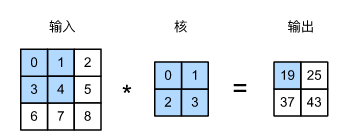
\includegraphics[width=\textwidth]{pic/Con_layer.png}
	\caption{卷积操作示意}
	\label{Con_layer}
\end{figure}

\subsection{激活层}

神经网络中的每个神经元,本层需要接受上一层的输出值作为本层神经元的输入值,并将输入值传递给下一层,输入层神经元节点会将输入属性值直接传递给下一层。因此在多层神经网络中,上层节点的输出和下层节点的输入之间存在一个函数关系,这个函数在神经网络结构中称为激活函数。而在实际运用过程中,激活函数的另一个作用就是,通过限制输出的数值范围,来使得神经网络结构的运算更简便。如图\ref{relu}所示,显示的是三种常见的激活函数,第一是RELU激活函数的数值范围在$[0, + \infty )$之间,第二是Sigmoid激活函数的数值范围为$(0,1)$,第三是Tanh激活函数的数值范围在$(-1,1)$ 之间。这三类激活函数最适合于神经卷积网络的传播过程,特别是RELU激活函数,广泛地运用在卷积神经网络的工程中。

\begin{figure}[h]
	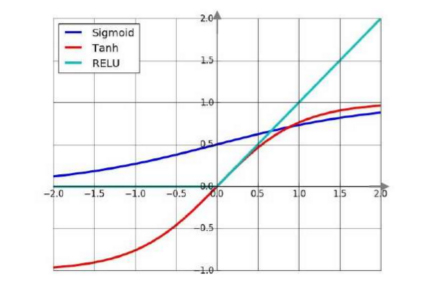
\includegraphics[width=\textwidth]{pic/relu.jpg}
	\caption{三种常见激活函数的对比示例}
	\label{relu}
\end{figure}

\subsection{池化层}

不同于卷积层就是将输入和卷积核进行互相关操作,池化层的作用则是直接计算滑动窗口内元素的最大值或者平均值,其本质其实就是降采样处理。目前学术界,对于池化而言,就是进行最大池化或者平均池化。池化层最大的优势就是在于防止出现训练过程中的过拟合问题,使得模型可以抽取更广泛的特征。

\subsection{批量归一化层}

对于浅层模型而言,标准化的预处理就已经足够满足需求啦。但是对于那些复杂的模型,当训练参数需要不断更新的时候,接近输出层的最终结果很难出现些许变化,很难训练出有效的神经网络结构。因此批归一化层的出现,就是要让这样深一点的神经网络结构的训练更加轻松容易。

在模型训练时,批量归一化计算小批量上的均值和标准差,不断调整神经网络的中间输出,从而使整个神经网络在各层的数值更稳定。

训练时,假设一个批量数据为$B = \{ {x_1},{x_2},...,{x_m}\}$,首先需要统计批量数据的的均值${\mu_B}$和方差$\sigma _B^2$,然后学习尺度参数$\gamma$和偏移参数$\beta$,将数据分布使其归一化${y_i} = \gamma \mathop {{x_i}}\limits^ \wedge   + \beta$

训练过程的计算步骤如下:
\begin{equation}
{\mu _B} = \frac{1}{m}\sum\limits_{i = 1}^m {{x_i}}
\end{equation}

\begin{equation}
\sigma _B^2 = \frac{1}{m}\sum\limits_{i = 1}^m {{{\left( {{x_i} - {\mu _B}} \right)}^2}}
\end{equation}

\begin{equation}
{\widehat x_i} = \frac{{{x_i} - {\mu _B}}}{{\sqrt {\sigma _B^2 + \varepsilon } }}
\end{equation}

\begin{equation}
{y_i} = \gamma \widehat {{x_i}} + \beta  = \gamma \frac{{{x_i} - {\mu _B}}}{{\sqrt {\sigma _B^2 + \varepsilon } }} + \beta
\end{equation}

在进行测试的环节时,因为测试样本数量较少,可以用于统计均值和方差不够用,所以需要对每批数据的期望值都要进行一定的归一化处理,测试的计算步骤如下:

\begin{equation}
E(x) = {E_B}\left[ {{\mu _B}} \right]
\end{equation}

\begin{equation}
Var[x] = \frac{m}{{m - 1}}{E_B}[{\mu _B}]
\end{equation}

\begin{equation}
y = \frac{\gamma }{{\sqrt {Var[x] + \varepsilon } }}x + (\beta  - \frac{{\gamma E(x)}}{{\sqrt {Var[x] + \varepsilon } }})
\end{equation}

\subsection{输入通道和输出通道}

对于一个图像而言,其包含的真实信息维度非常高。举个例子,彩色图像不只是只有高和宽这两个维度,实际上还包括RGB三个通道。假设高为H像素,宽为W像素,那么对于该图像而言,可以将其表示成一个3*H*W的多维数组,这第三维即叫做通道数。

在实际运用过程中,如果当输入数据1包含多个通道时,需要设计一个与输入通道数相匹配的卷积核,这样的话就能和多通道的输入数据做互相关运算啦。分析可知,输入数据的通道数为$c_i$,那么卷积核的输入通道数同样为$c_i$。设卷积核窗口尺寸为${k_h} \times {k_w}$。当${c_i} = 1$时,那么卷积核只包含一个尺寸为${k_h} \times {k_w}$	
 的二维数组。当${c_i} > 1$时,每个输入通道各分配一个尺寸为${k_h} \times {k_w}$的卷积核数组。把这$c_i$个数组在输入通道维上连结,即得到一个尺寸为${c_i} \times {k_h} \times {k_w}$的卷积核。由于输入和卷积核各有$c_i$	
 个通道,将每一个通道上的二维数组和卷积核的二维数组做互相关运算,再将这$c_i$个互相关运算的二维输出按通道相加,得到一个二维数组。
 
如图\ref{2_chan_input}所示,展示了含2个输入通道的二维互相关计算的例子。

\begin{figure}[h]
	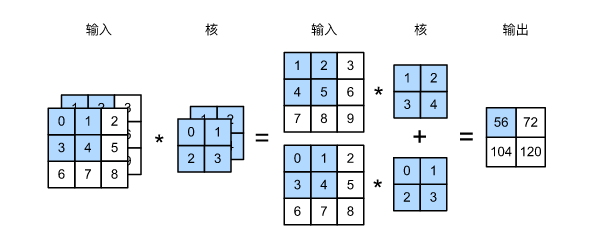
\includegraphics[width=\textwidth]{pic/2_chan_input.png}
	\caption{含2个输入通道的互相关运算}
	\label{2_chan_input}
\end{figure}

当输入通道有多个时,因为我们对各个通道的结果做了累加,所以不论输入通道数是多少,输出通道数总是为1。

\section{沙漏网络结构}

本文算法采用,沙漏网络的结构来进行人体姿态估计。该模型非常适用于人体检测任务,在MPII竞赛中获得了第一名。串联的堆叠沙漏网络复用全身关节信息,来提高对于单个关节的识别精度,后面会做进一步解释。

\subsection{残差模块}

残差模块是堆叠沙漏网络的基础模块,其原理如下:

残差网络原理如下:设输入为x,假设对于网络结构而言,理想映射为f(x)。\ref{Res_module}左图需要直接设计出该映射f(x),但是右图则需要直接设计出残差映射$f(x) \to x$。在实际情况下,残差映射更容易优化。

\begin{figure}[h]
	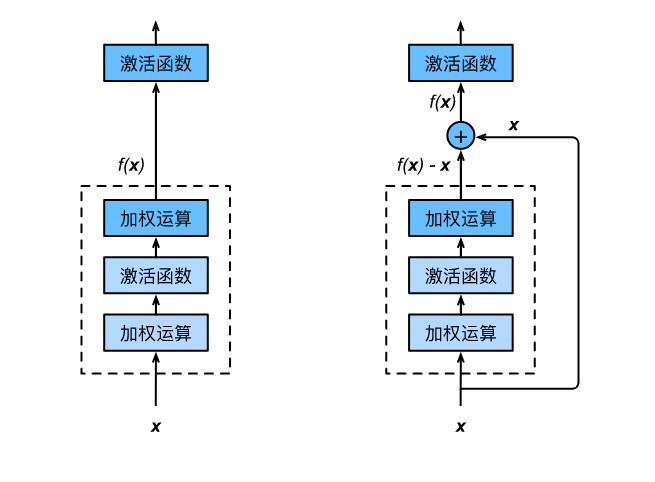
\includegraphics[width=0.8\textwidth]{pic/Res_module.jpg}
	\caption{普通的网络结构(左)与加入残差连接的网络结构(右)}
	\label{Res_module}
\end{figure}

堆叠沙漏网络结构采用了残差模块作为其基本单元,其基本结构如图所示,有主路与旁路两部分。其参数采用\citing{DBLP:journals/corr/NewellYD16}论文里设置的原始参数,这里不做更改。如图\ref{res_net}所示,主路部分上有三个尺寸分别为1*1,3*3,1*1的卷积核。旁路部分则只有一个1*1的卷积核构成,起着卷积层的作用,可以保留原始信息。然后批归一化层和激活层都作用在每一个卷积层的输入处。这也就是说,特征图在通过沙漏网络之后,并不会改变其尺寸,本质上而言,只有通道数发生了变化。

假设输入图像的通道数为M,输出图像的通道为N,则主路部分的第一个卷积层和第二个卷积层的卷积核数量都是N/2,第三个卷积层的卷积核数量为N。

其中,$M \to N$代表整个网络输入的通道数为$M$,通过网络输出的通道数转变为$N$,$w$表示设置的网络权重,$b$表示设置的偏置。

\begin{figure}[h]
	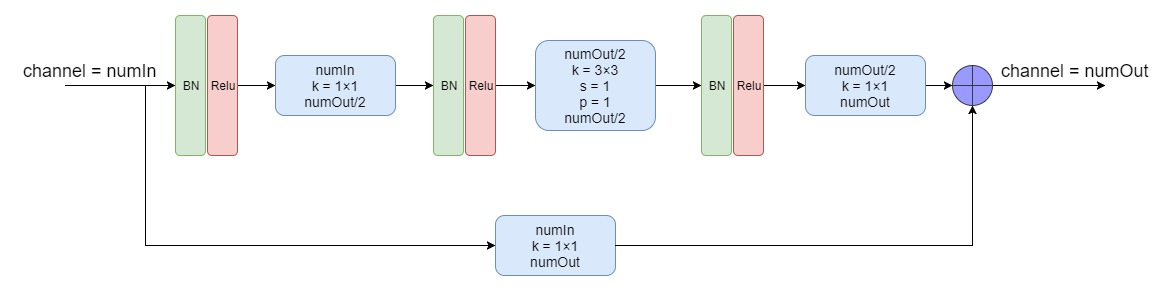
\includegraphics[width=\textwidth]{pic/res_net.jpg}
	\caption{残差模块}
	\label{res_net}
\end{figure}

\subsection{一阶沙漏网络}

\citing{DBLP:journals/corr/NewellYD16}论文介绍,一阶沙漏网络就是基于残差模块设计的,也有主路和旁路两部分,如图\ref{1_hg}所示。\citing{黄铎2019基于}对于主路部分而言,通过最大池化层,提取输入图像的特征信息并缩小图片尺寸。对于旁路而言,主要是保留输入图像的各关节点的特征信息。整体而言,使得网络在不同尺寸下的图片下都可以提取关节点的信息,而上采样可以将特征图恢复到原始尺寸,并与旁路的输出相加,最终完成提取特征的目标。输入图像提取的特征值用x来表示。其中maxpool()表示最大池化层,unsampling()表示上采样层。

\begin{equation}
y_{M \to N}^1(x) = {f_{256 \to N}}({f_{256 \to 256}}({f_{256 \to M}}(x))) + upsampling({f_{N \to N}}(...({f_{M \to 256}}(\max pool(x))))
\end{equation}

\begin{figure}[h]
	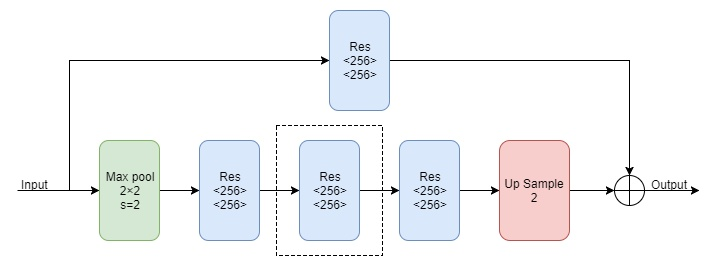
\includegraphics[width=\textwidth]{pic/1_k_hourglass.jpg}
	\caption{一阶沙漏网络}
	\label{1_hg}
\end{figure}

\subsection{二阶沙漏网络}

设计二阶沙漏网络时,只需要将一阶沙漏网络中,主路的一个残差模块替换成另一个一阶沙漏网络,如图\ref{2_hg}所示,就可以得到二阶沙漏网络。图中上下箭头分别表示上下采样,$H$和$W$分别表示输入图像的高和宽像素值,$M$和$N$分别表示整体网络输入和输处的通道数。

分析可知,在每次通过最大池化层之前,每个关节点的空间位置信息都会输入到旁路的卷积层,而且有两个残差模块来提取特征,这也就是说,二阶沙漏网络可以提取出初始,1/2,1/4尺寸的关节点特征。通过上采样使得图像尺寸恢复到与旁路相同尺寸大小,这样再进行特征融合后,即可完成目标任务。

\begin{figure}[h]
	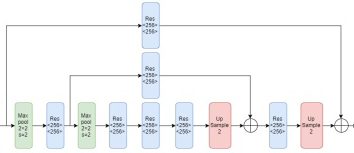
\includegraphics[width=\textwidth]{pic/2_k_hourglass.jpg}
	\caption{二阶沙漏网络}
	\label{2_hg}
\end{figure}

\subsection{四阶沙漏网络}

如法炮制,在设计四阶沙漏网络时,只需要将二阶沙漏网络中,主路的一个残差模块替换成另一个二阶沙漏网络,就可以得到一个四阶的沙漏网络。如图\ref{4_hg}所示的四阶沙漏网络。

\begin{figure}[h]
	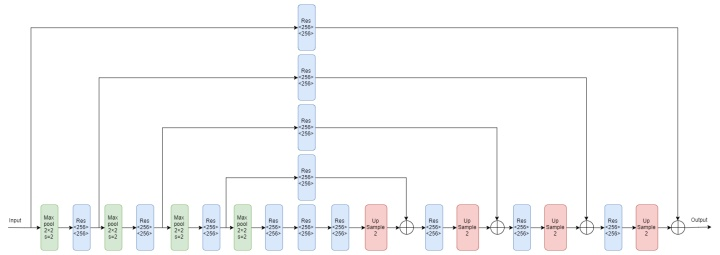
\includegraphics[width=\textwidth]{pic/4_k_hourglass.jpg}
	\caption{四阶沙漏网络}
	\label{4_hg}
\end{figure}

分析可知,对于四阶沙漏网络而言,在每次通过最大池化层之前,每个关节点的空间位置信息都会输入到旁路的卷积层,而且有两个残差模块来提取特征,这也就是说,四阶沙漏网络可以提取出初始,1/2,1/4,1/8尺寸的关节点特征。通过上采样使得图像尺寸恢复到与旁路相同尺寸大小,这样再进行特征融合后,即可完成目标任务。

\subsection{高阶沙漏网络}

本文算法采用了高阶堆叠沙漏网络作为人体姿态估计的主干检测网络。

以此类推,高阶堆叠沙漏网络在numReductions>1时,递归调用自己。

其设计的迭代思路如图\ref{8_k_hourglass}所示。

\begin{figure}[h]
	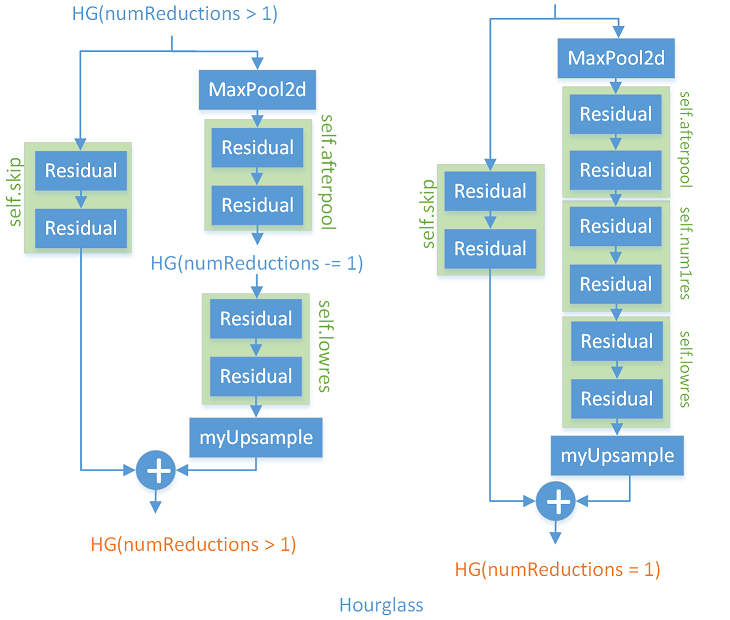
\includegraphics[width=\textwidth]{pic/8_k_hourglass.png}
	\caption{高阶沙漏网络迭代逻辑}
	\label{8_k_hourglass}
\end{figure}

\subsection{中间监督}

整个堆叠沙漏网络可以不断进行上采样和下采样的过程,\citing{DBLP:journals/corr/NewellYD16}提到这种结构的关键在于中间监督,能够对每一个沙漏模块的性能以及数据进行预测分析,在实际工程中,即在中间层级处,利用热力图计算损失。关于中间监督的位置,作者在文中也进行了讨论。对于大多数高阶特征而言,仅会在较低的分辨率下出现。如果监督再网络上采样之后,就很难在更大的全局中重新评估这些特征;如果网络能够得到最好的预测,在一个局部范围内进行的预测就很没有必要。由于沙漏网络模块整合了局部和全局的信息,若想要网络在早期进行预测,则需要它对图片有一个高层次的理解即使只是整个网络的一部分。最终,作者将中间监督设计在如下图所示位置:\ref{intermediate_supervision}

网络分裂并产生一组热力图(蓝色轮廓),其中可以应用1x1卷积,重新映射热力图,以匹配中间特征的通道数。这些是与前面沙漏模块的特征一起添加的。

\begin{figure}[h]
	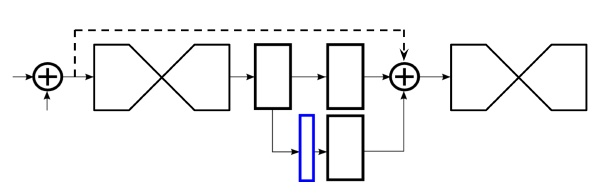
\includegraphics[width=\textwidth]{pic/intermediate_supervision.jpg}
	\caption{中间监督}
	\label{intermediate_supervision}
\end{figure}

\subsection{2D人体姿态估计算法框架的思路}

卷积神经网络的输入的图片分辨率为256×256,在沙漏网络模块中的最大分辨率为64×64,因此整个网络最开始要经过一个7×7的步长为2的卷积层,之后再经过一个残差块和最大池化层使得分辨率从256降到64。

整个算法框架只能用于单人姿态检测,但是在一张图片中经常有多个人,解决办法就是利用标签文件设计一个包围框范围,将包围框中的关节点数据判定为一个目标任务。再将目标人物裁剪到正中心后再将输入图片调整大小到256×256。整个网络使用RMSprop进行优化,学习率为2.5e-4. 测试的时候使用原图及其翻转的版本进行预测,结果取平均值。网络对于关节点的预测是热力图的最大激活值。损失函数使用均方误差(Mean Squared Error,MSE)来比较预测的heatmap与ground truth的heatmap(在节点中心周围使用2D高斯分布,标准差为1)

\begin{equation}
MSE = \frac{1}{n}\sum\limits_{i = 1}^n {{{\left( {\widehat {{x_i}} - {x_i}} \right)}^2}}
\end{equation}

\section{本章小结}
本章首先介绍了人体姿态估计中常见的深度学习技术,包括卷积神经网络各层的含义,以及输入通道和输出通道的概念。然后介绍了残差模块,沙漏模块,堆叠沙漏网络的设计原理。最后得出2D人体姿态估计算法框架的思路。
